\documentclass[notheorems,16pt,utf8,fullscreen=true,bookmarks=false]{beamer}
\usepackage{../Styles/Personal_data}

\usepackage[english,russian]{babel}
\usepackage[utf8]{inputenc}
\usepackage{pscyr}
\usefonttheme[onlymath]{serif}
\usepackage{amsfonts,amsmath}
\usepackage{cite,enumerate,float,indentfirst}

\usepackage{xcolor}

\usepackage{graphicx}
\usepackage{caption}
\usepackage{ragged2e}
\usepackage{pgfpages}

\usepackage{multirow} %объединение строк в таблицах
\usepackage{tabularx}

\parskip=0.25cm
\pgfpagesuselayout{resize to}[a4paper,border shrink=5mm,landscape]
\definecolor{chromeyellow}{rgb}{1.0, 0.65, 0.0}

\captionsetup{labelsep=period}
\justifying
\renewcommand{\raggedright}{\leftskip=0pt \rightskip=0pt plus 0cm}
\setbeamersize{text margin left=0cm, text margin right=0cm}
\setbeamertemplate{navigation symbols}{}
\setbeamercolor{alert}{bg=chromeyellow}


\graphicspath{{../Images/}}   

\usetheme[]{Boadilla}

\setbeamertemplate{blocks}[rounded][shadow=false]
\addtobeamertemplate{block begin}{\pgfsetfillopacity{0.8}}{\pgfsetfillopacity{1}}
\setbeamercolor{structure}{fg=black}
\setbeamercolor{frametitle}{bg=chromeyellow!50!white}
\setbeamertemplate{enumerate items}[circle]
\setbeamertemplate{itemize items}[circle]

\setbeamerfont{frametitle}{size=\large\bf}

\beamertemplatenavigationsymbolsempty

\setbeamercolor{footline}{fg=gray}
\addtocounter{framenumber}{-1}
\setbeamertemplate{headline}{}
\setbeamertemplate{footline}{
  	\leavevmode%
  	\hbox{%
  		\begin{beamercolorbox}[wd=.333333\paperwidth,ht=2.25ex,dp=1ex,center]{}%
    		\small \student
  		\end{beamercolorbox}%
  		\begin{beamercolorbox}[wd=.333333\paperwidth,ht=2.25ex,dp=1ex,center]{}% 
  		\end{beamercolorbox}%
  		\begin{beamercolorbox}[wd=.333333\paperwidth,ht=2.25ex,dp=1ex,right]{}%
			\small Слайд \insertframenumber{} \hspace{1cm} 
  		\end{beamercolorbox}}%
  	\vskip0pt%
	}
\newtheorem{theorem}{Теорема}

\begin{document}
{
\setbeamertemplate{footline}{} 
\begin{frame}
% Логотип университета и название 
		\begin{minipage}[h]{0.1\linewidth}
			\begin{center}
				
\includegraphics[scale=0.15]{lstu_logo.jpg}		
			\end{center} 
		\end{minipage}
		\hfill
		\begin{minipage}[h]{0.8\linewidth}
			\begin{center}
				 {\LARGE\scshape\bf Липецкий государственный технический университет}
			\end{center}
		\end{minipage}
			
		\begin{center}
			\large\textbf{\studentIm} \\ 
			\vspace{1cm}
			\thema \\
			\vspace{1cm}
			\normalsize Направление \major \\
		\end{center}
		\vspace{0.5cm}
		\begin{minipage}[h]{0.54\linewidth}
			\begin{center}
				Научный руководитель \\
				\ad 
			\end{center} 
		\end{minipage}
		\hfill
		\begin{minipage}[h]{0.4\linewidth}
		\begin{center}
			\small \adviser
		\end{center}
		\end{minipage}
\end{frame}
}
\normalsize
% ======== Slide 1 =========
\begin{frame}
\frametitle{Цель и задачи}
	\textbf{Актуальность (опционально)} ....
	
	\textbf{Цель работы --} ..... 
	
	\textbf{Задачи:} ..... 
	
   	\begin{itemize}
   		\item ...
   		\item ...
   		\item ...
   	\end{itemize}
\end{frame}


% ======== Slide 2 =========

\begin{frame}
\frametitle{Название слайда}
Пример многоуровневого списка

\begin{enumerate}
  \item \textbf{Задача 1}
  \begin{itemize}
    \item Подзадача 1-1
    \item Подзадача 1-2
  \end{itemize}
  \item \textbf{Задача 2}
  \begin{itemize}
    \item Подзадача 2-1
    \item Подзадача 2-2
    \item Подзадача 2-3
  \end{itemize}
  \item \textbf{Задача 3}
  \begin{itemize}
    \item Подзадача 3-1
    \item Подзадача 3-2
    \item Подзадача 3-3
  \end{itemize}
\end{enumerate}
\end{frame}

% ======== Slide 3 =========

\begin{frame}
\frametitle{Название слайда}
Пример размещения текста и нескольких рисунков
	\begin{center}
	\begin{minipage}[h]{0.39\linewidth}
		\begin{center}
			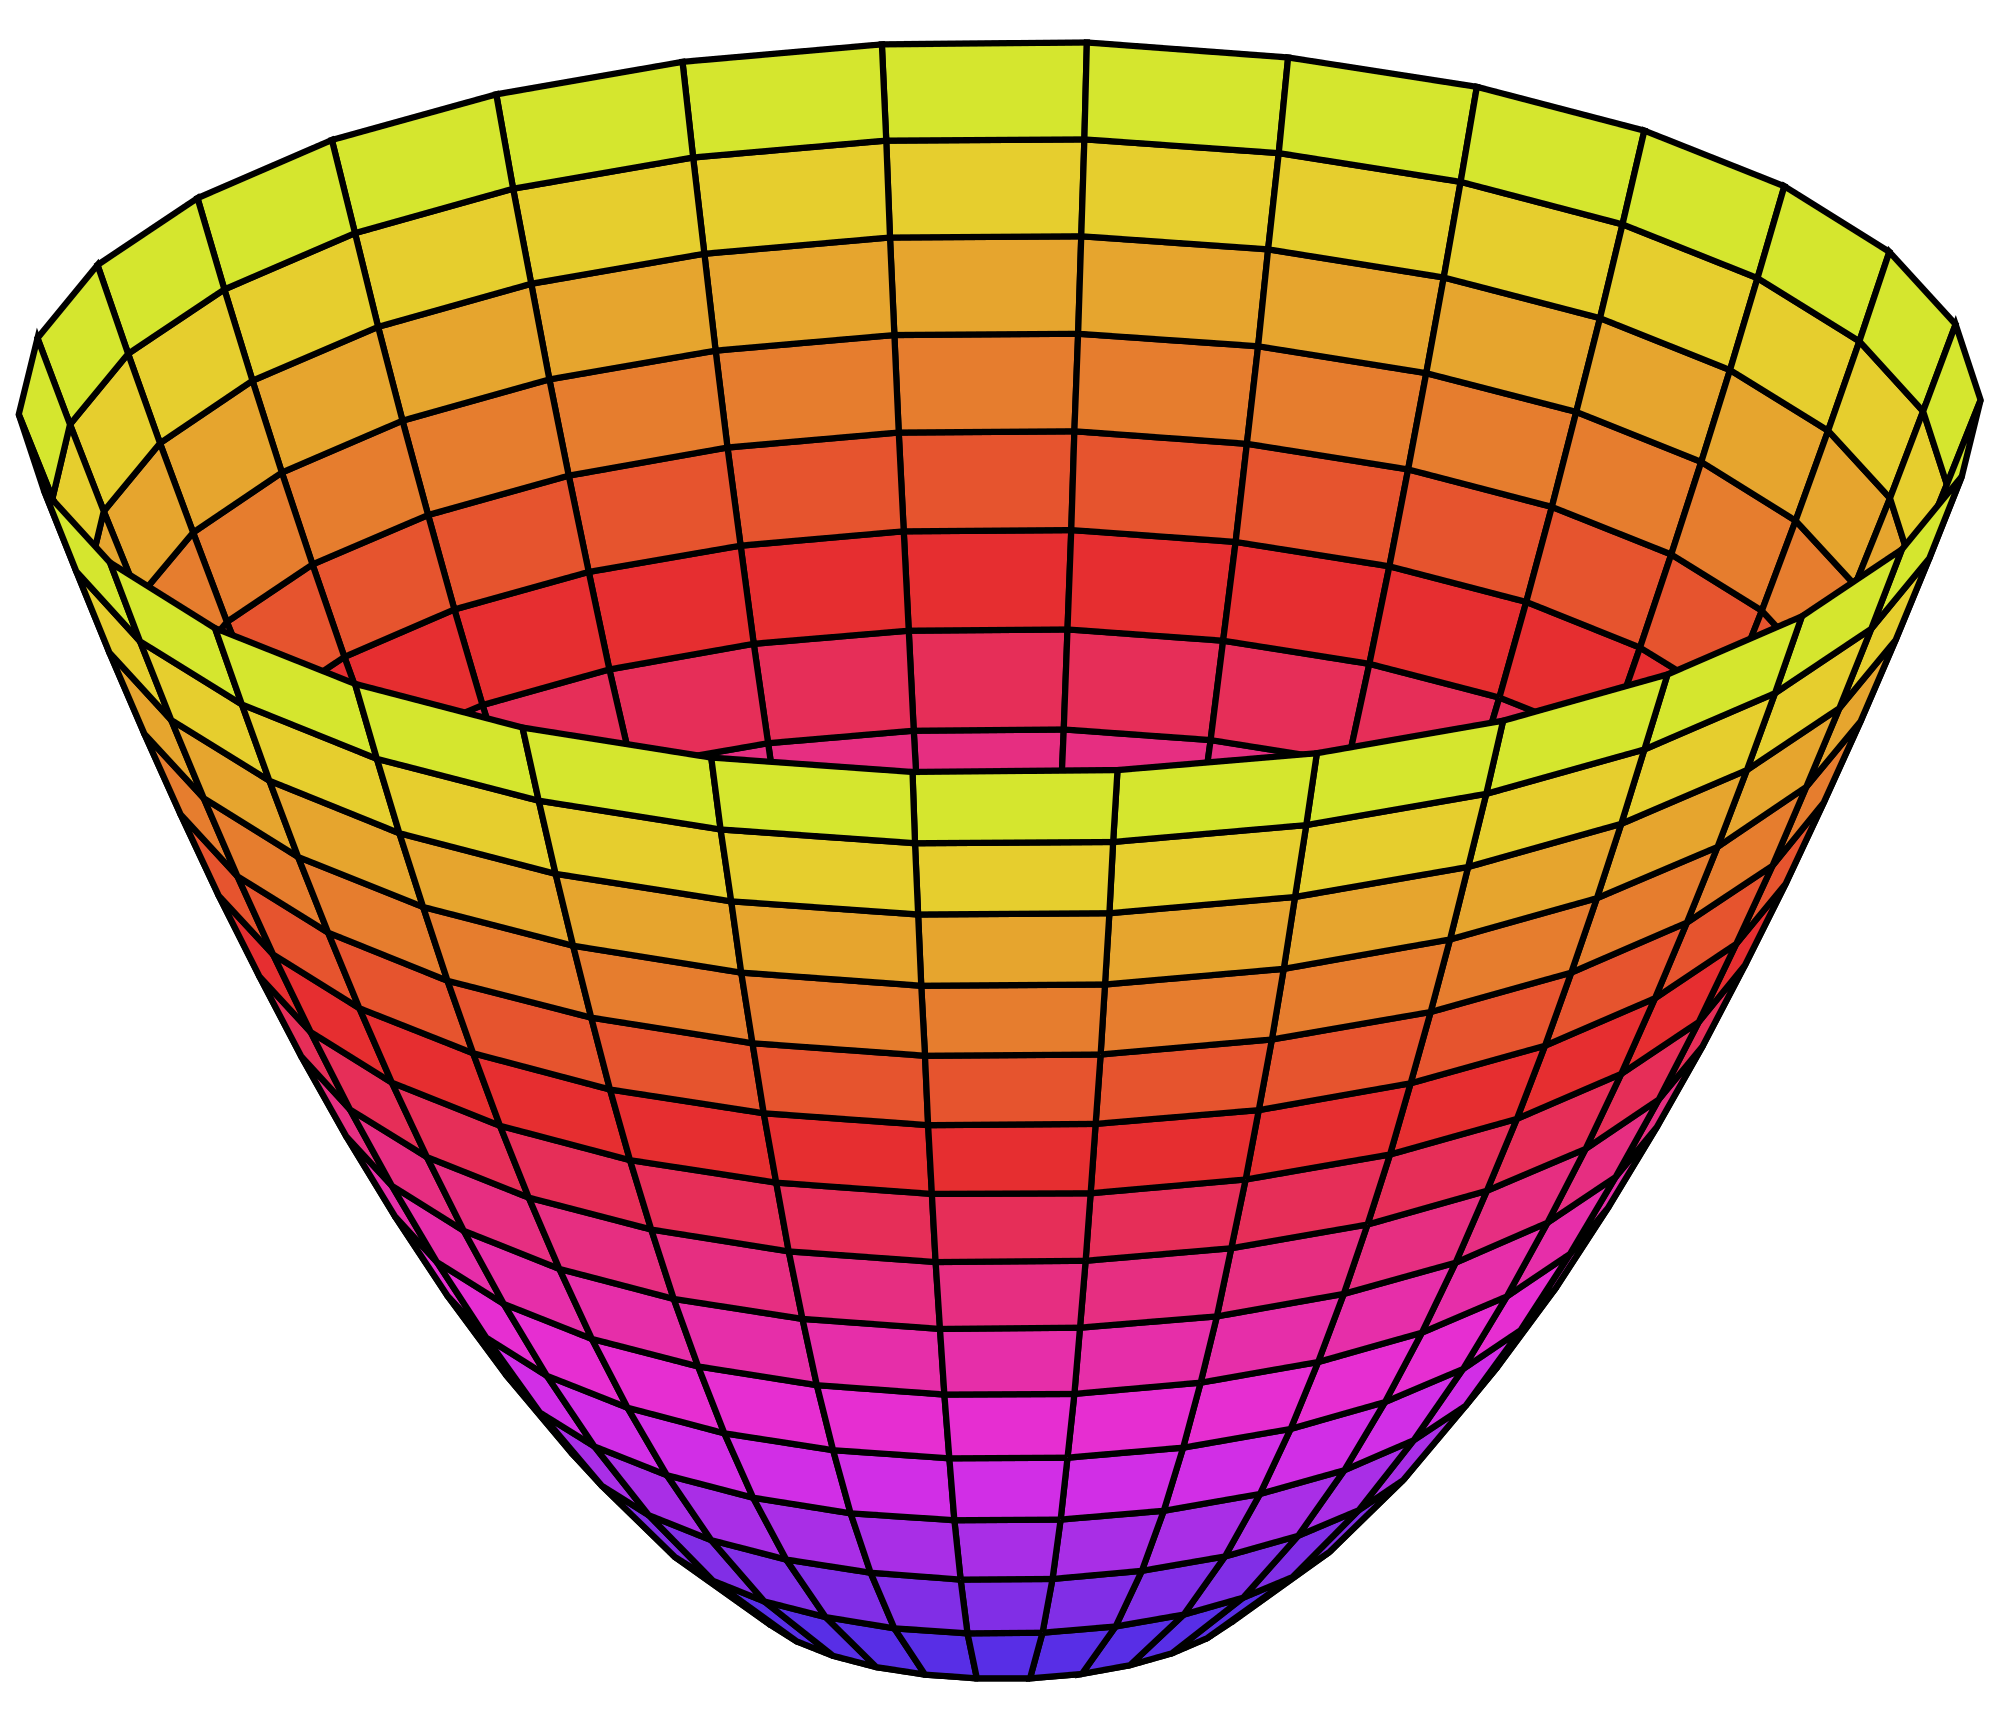
\includegraphics[scale=0.065]{paraboloid.png}
			
			\small Рисунок 1 --- Параболоид	
		\end{center}
	\end{minipage}
	\hfill 
	\begin{minipage}[h]{0.59\linewidth}
		\begin{center}
			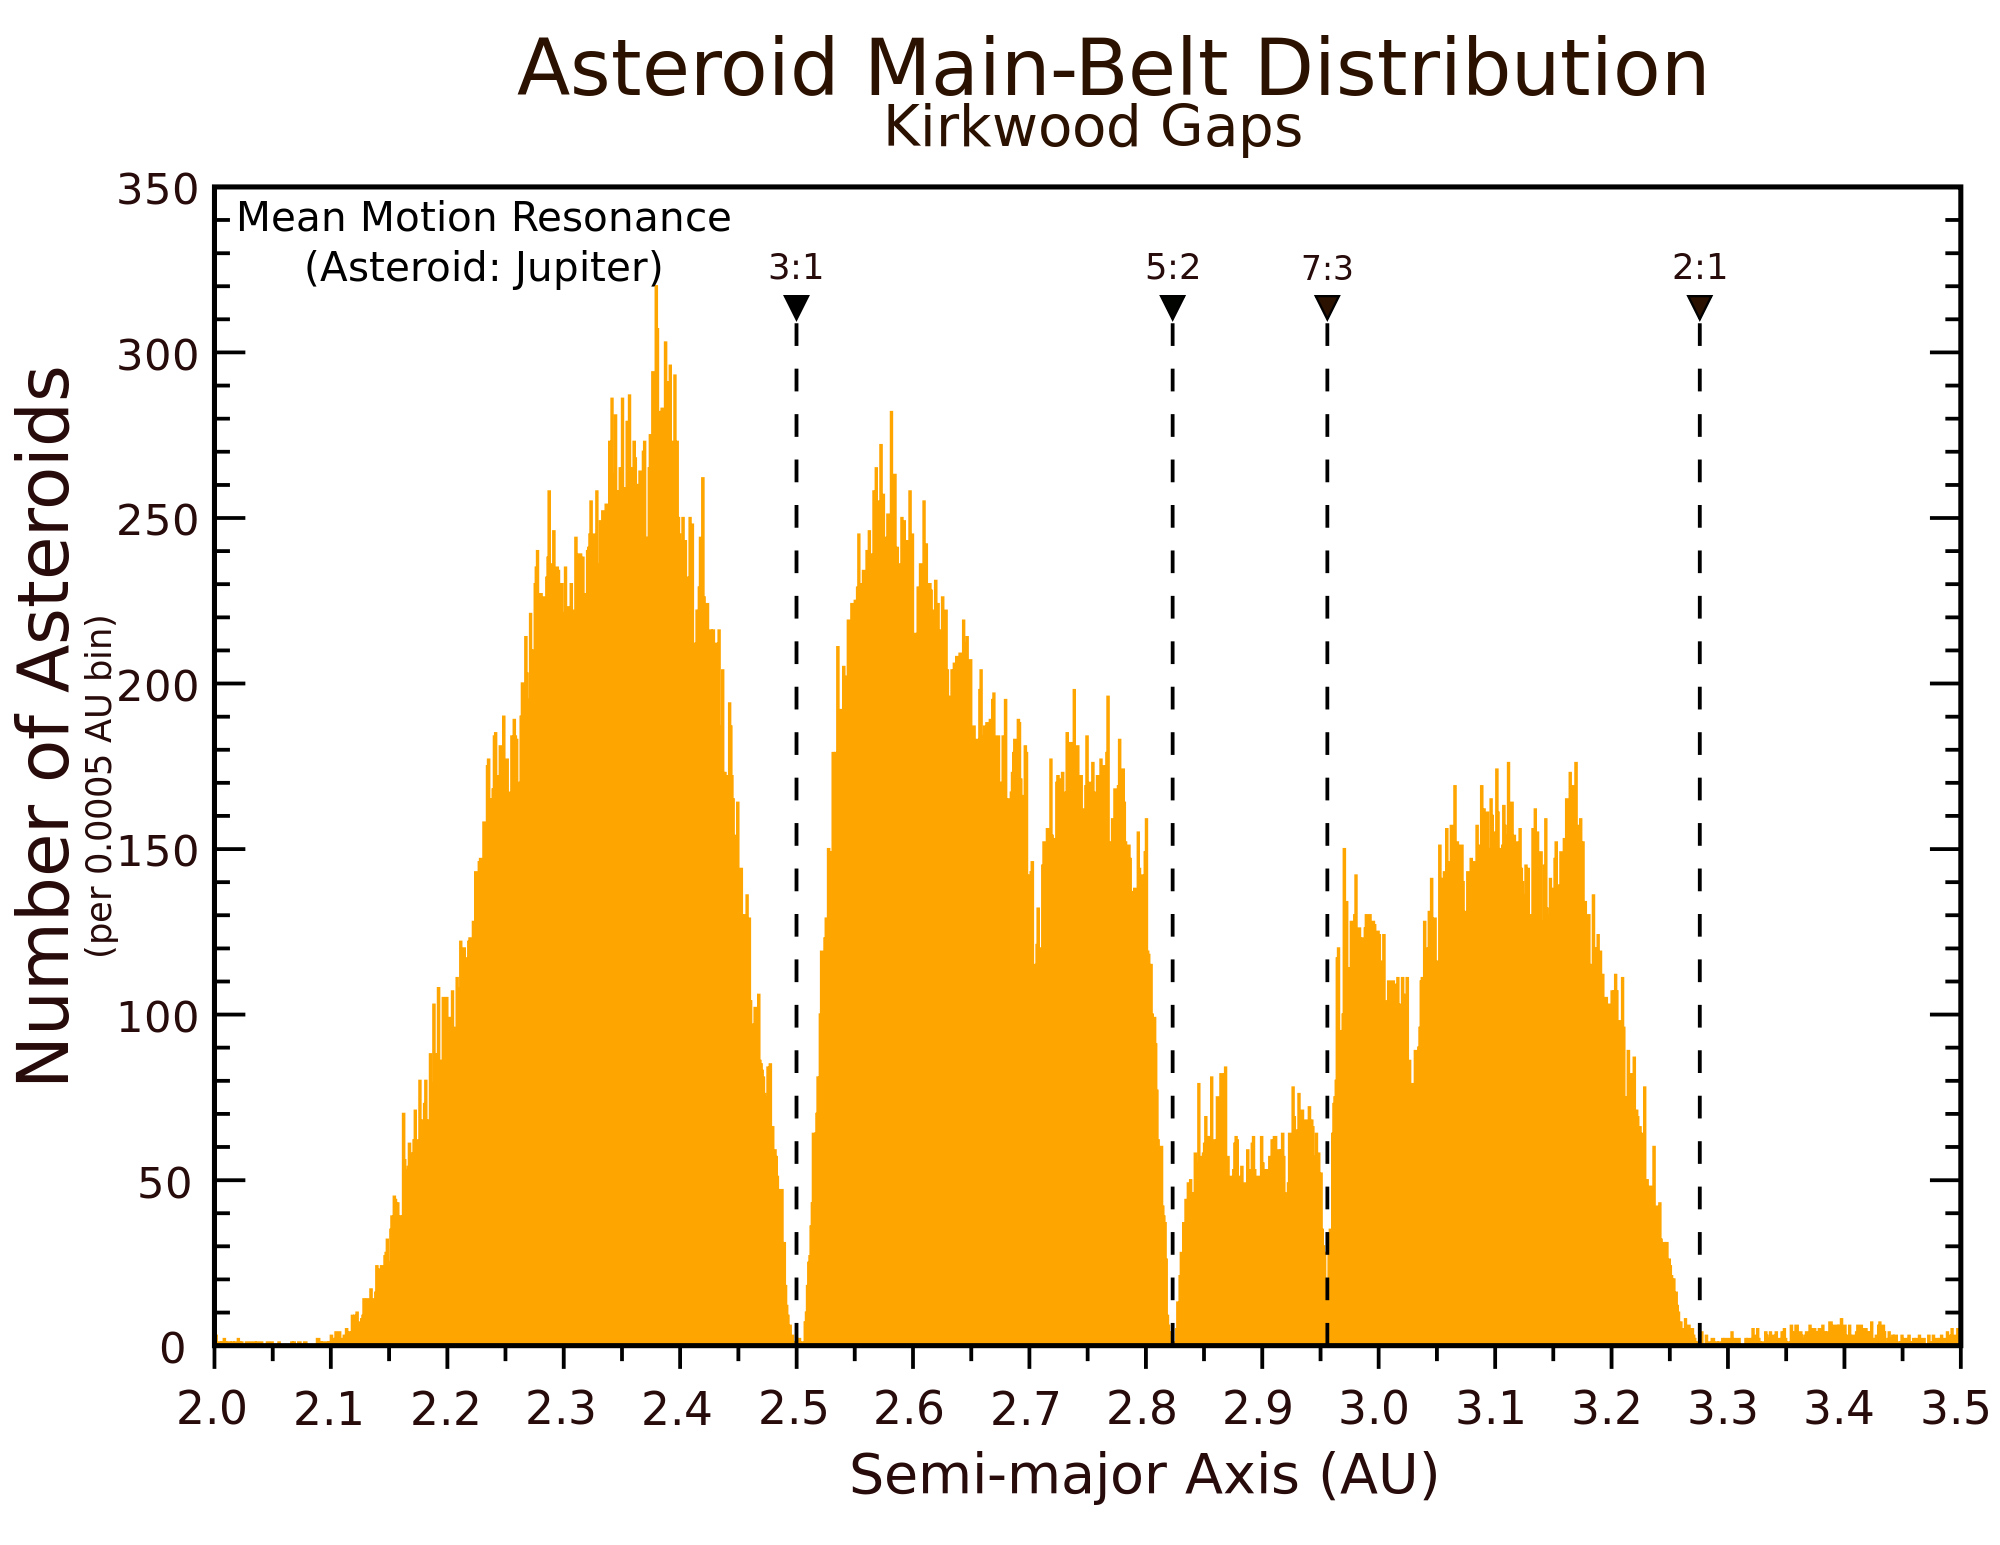
\includegraphics[scale=0.075]{distribution.png}
			
			\small Рисунок 2 --- Пример распределения
		\end{center}
	\end{minipage}
	\end{center}

\end{frame}

% ======== Slide 4 =========

\begin{frame}
\frametitle{Пример таблицы}
	\begin{center}
		\begin{center}
		Таблица 1 --- Название таблицы
		\end{center}
		\small
		\begin{tabularx}{\textwidth}{|X|X|X|X|X|}
			\hline 
			\multirow{2}{*}{Головка} 
			& \multicolumn{2}{c|}{Графа 1} & \multicolumn{2}{c|}{Графа 2} \\
			\cline{2-5}
  			& Подграфа 1 & Подграфа 2 & Подграфа 3 & Подграфа 4 \\ 
			\hline
  			&   &   &   &  \\ 
			\hline
  			&   &   &   &  \\ 
			\hline 
		\end{tabularx}
	\end{center}
\end{frame}

% ======== Slide 5 =========

\begin{frame}
\frametitle{Формулы}
	\label{r1}
	\begin{equation}
	\left\{
  		\begin{array}{rl}
    	\dot x = & \sigma (y-x), \\
    	\dot y = & x (r - z) - y, \\
    	\dot z = & xy - bz.
  	\end{array} \right.
	\end{equation}
	\begin{eqnarray}
	l \quad I
	\end{eqnarray}
\end{frame}


% ======== Slide n =========

\begin{frame}
\frametitle{Публикации (при наличии)}
	\vspace{0.5cm}
	\begin{enumerate}
		\item Публикация 1
		\item Публикация 2
		\item Публикация 3
	\end{enumerate}
	\vspace*{10cm}
\end{frame}


\setbeamertemplate{headline}{}
\begin{frame}
	\begin{center}
		\LARGE Спасибо за внимание!
	\end{center}
\end{frame}

\end{document} 